\begin{figure}[t]
 	\centering
	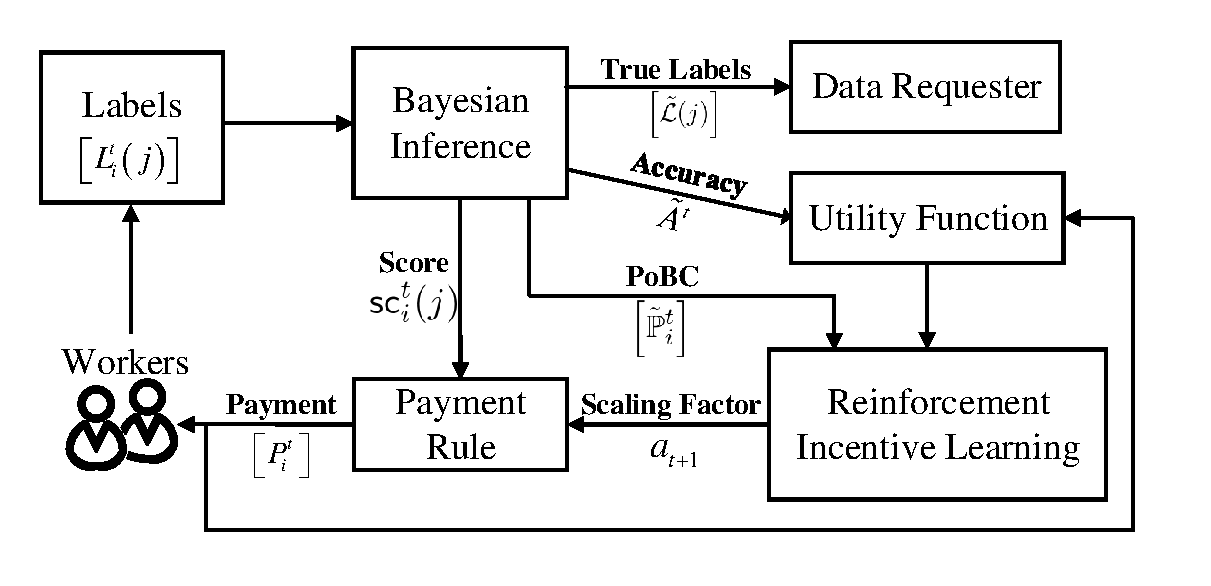
\includegraphics[width=0.48\textwidth]{image/Architecture}
	\vspace*{-8mm}
    \caption{\label{Archi} Architecture of our incentive mechanism}
\end{figure}
\section{Incentive Mechanism for Crowdsourcing}
We present the architecture of our incentive mechanism in Figure~\ref{Archi}, where the estimate of a variable is denoted by adding an over-tilde.
In our incentive mechanism, the Bayesian inference algorithm is responsible for estimating the true labels, workers' PoBCs and the label accuracy based on the collected labels at each time step.
The payment rule is designed to ensure that reporting truthfully ($r^{t}_i = 0$) and exerting high efforts ($e^{t}_i=1$) is the payment-maximizing strategy for all workers at any time step.
By doing so, we wish to induce workers to generate high-quality labels and thus improve the label accuracy.
The reinforcement adjustment algorithm adjusts the payment rule based on the historical data of payments, workers' PoBCs and label accuracy.
In this way, we can optimally balance the utility got from the labels and lost in the payments, which corresponds to $F(A^t)$ and $\sum_{i}P_i^t$ in Equation~\ref{utility}, respectively.
Besides, our incentive mechanism can ensure that always reporting truthfully ($r^{t}_i \equiv 0$) and exerting high efforts ($e^{t}_i \equiv 1$) is the payment-maximizing strategy for workers in the long term.
This property prevents the clever manipulation which earns higher long-term benefits by sacrificing short-term ones.

Nevertheless, there are three challenges to achieve our design. Firstly, our empirical studies reveal that popular inference algorithms may be heavily biased on estimating the label accuracy when the quality of labels is very low. For example, when there are $10$ workers and $q_i^t=0.55$, the estimated label accuracy of the EM estimator~\cite{dawid1979maximum,raykar2010learning} stays at around $0.9$ while the real accuracy is only around $0.5$.
This heavy bias will cause the utility to be miscalculated and thus mislead our reinforcement adjustment.
To reduce the inference bias, we develop our Bayesian inference algorithm by introducing the soft Dirichlet priors for both the true labels and workers' PoBCs.
In this case, the posterior distribution cannot be expressed as any known distributions, which motivates us to derive the explicit posterior distribution at first and then employ Gibbs sampling to conduct inference.
{\color{red}Secondly, the reinforcement adjustment expects the utility to be accurately calculated so that the direction of adjustment is clear.
However, both the label accuracy and workers' PoBCs in our incentive mechanism are corrupted by noise.
Considering that these estimates are calculated as an average over $M$ tasks, the central limit theorem ensures that the inference noise approaches the Gaussian distribution.
Therefore, to overcome the inference noise, we develop our reinforcement adjustment algorithm based on the Gaussian process.}
Lastly, the biggest challenge of our study is to prove that our incentive mechanism can ensure that reporting truthfully and exerting high efforts is the payment-maximizing strategy for workers in not only each time step and but also the long term.
For clarity, we put the theoretical analysis in the next section.
In this section, we focus on the first two challenges.


%Figure~\ref{Archi} shows the architecture of our incentive framework.
%Different from industrial feedback control systems, crowdsourcing markets require the data requester to announce the incentive mechanism to workers before allocating tasks to workers, which is actually a contract between two sides.
%So, we design our framework as two levels.
%The inner level is the Bayesian incentive mechanism which is always open to workers.
%Its objective is to ensure that reporting truthfully and exerting high efforts are the optimal strategy for all workers at any time step $t$.
%By doing so, we expect that all workers are fully rational and can follow this optimal strategy.
%However, in practice, human workers may not always fully rational and can even learn from the interactions with our mechanism.
%Thus, we develop the outer level, the reinforcement incentive mechanism, which adjusts the scaling level $a^t$ of our Bayesian mechanism to maximize the long-term utility of the data requester.
%Meanwhile, our reinforcement incentive mechanism must also ensure that reporting truthfully and exerting high efforts are the optimal strategy for workers in the long term.
%In this way, we can prevent the manipulation of any single worker.




\subsection{Payment Rule}
Suppose, at time step $t$, worker $i$ finishes $M^{t}_{i}$ tasks.
Then, the payment for worker $i$ should be
\begin{equation}
P^t_i=M_i^t\cdot (a^t r^{t}_i+b)\;\; , \;\; \phi^{t}_i = \tilde{p}^{t}_i - 0.5
\end{equation}
where we call $\phi^{t}_i$ as worker $i$'s score and $\tilde{p}^{t}_i$ will be calculated by our Bayesian inference algorithm.
$a^t$ is the scaling factor. 
It is determined by our reinforcement adjustment algorithm at the beginning of step $t$.
We denote all the available values of $a^t$ as set $\mathcal{A}$.
Besides, $b\geq 0$ is the fixed base payment.


\subsection{Bayesian Inference}
%An accurate inference algorithm, which is responsible for estimating $L^{t}(j)$, $p^t_i$ and $A^t$, is the foundation of our framework. There have been many inference algorithms developed in the literature~\cite{zheng2017truth}. Among them, two popular ones are the EM estimator~\cite{dawid1979maximum} and the variational inference estimator~\cite{liu2012variational}.
%However, our empirical studies in Figure~\ref{BIM1} reveal that these iterative estimators, which may converge to the local optimum, will be heavily biased when the quality of labels is very low.
%Thus, we employ the similar Dirichlet priors as the variation inference estimator but explicitly derive the posterior distribution of true labels rather than relying on the evidence lower bound~\cite{blei2017variational}.
%Then, we use Gibbs sampling to efficiently sample the posterior distribution to calculate the estimates of $L^{t}(j)$, $p^t_i$ and $A^t$.

%since the EM estimator may converge to the local optimum.
%On the other hand, sampling-based Bayesian inference algorithms, for example Gibbs sampling, are computationally very expensive, even though they use the explicit posterior distribution and can avoid the inference bias.
%Especially, workers' scores are continuous variables, which will significantly slow down the convergence speed.
%Therefore, to the best of my knowledge, sampling-based Bayesian inference is never used for crowdsourcing where the number of workers and tasks is usually very large.
%In this section, to reduce the inference bias and meanwhile avoid overly large computation costs, we firstly assume Dirichlet priors for those continuous variables in our system and derive a joint posterior distribution which only contains the discrete variables.
%Then, we use Gibbs sampling to sample the obtained posterior distribution and estimate workers' scores based on those samples.

%\footnote{In practice, $M^{t}_{i}$ is often smaller than $M$, and we can introduce $L^{t}_i(j)=0$ to denote that task $j$ is not assigned to worker $i$. The incentive mechanisms developed in this paper can work well in the case where the matrix $[L^{t}_i(j)]$ is sparse. However, to simplify the theoretical analysis, we assume $M^{t}_{i}\equiv M$ in this paper and put the theoretical analysis on the sparse case as our future work.}

Now, we present the details of our inference algorithm. For the simplicity of notations, we omit the superscript $t$ in this subsection. The joint distribution of the collected labels $\mathcal{L}=[L_i(j)]$ and the true labels $\bm{L}=[L(j)]$ satisfies
\begin{equation}
\label{JointDist}
\begin{split}
    &P(\mathcal{L},\bm{L}| \bm{p}, \bm{\tau})=\\ &\qquad {\prod}_{j=1}^{M}{\prod}_{k=1}^{K}\left\{\tau_{k}\prod_{i=1}^{N}p_i^{\delta_{ijk}}(1-p_i)^{\delta_{ij(3-k)}} \right\}^{\xi_{jk}}
\end{split}
\end{equation}
where $\bm{p}=[p_i]_N$ and $\bm{\tau}=[\tau_1,\tau_2]$. $\tau_1$ and $\tau_2$ denote the distribution of answer $1$ and $2$ among all tasks, respectively.
Besides,  $\delta_{ijk}=\mathbbm{1}(L_i(j)=k)$ and $\xi_{jk}= \mathbbm{1}(L(j)=k)$.
Here, we assume Dirichlet priors $\textrm{Dir}(\cdot)$ for $p_i$ and $\bm{\tau}$ as
\begin{equation}
[p_{i}, 1-p_i]\sim \textrm{Dir}(\alpha_{1},\alpha_{2})\;,\; \bm{\tau}\sim \textrm{Dir}(\beta_{1},\beta_{2}).
\end{equation}
Then, the joint distribution of $\mathcal{L}$, $\bm{L}$, $\bm{p}$ and $\bm{\tau}$ satisfies
\begin{equation}
\label{JointDist2}
\begin{split}
&P(\mathcal{L},\bm{L},\bm{p}, \bm{\tau}|\bm{\alpha}, \bm{\beta})=P(\mathcal{L},\bm{L}|\bm{p}, \bm{\tau})\cdot P(\bm{p}, \bm{\tau}|\bm{\alpha}, \bm{\beta})\\
&=\frac{1}{B(\bm{\beta})}\prod_{k=1}^{K}\tau_k^{\hat{\beta}_k-1}\cdot\prod_{i=1}^{N}\frac{1}{B(\bm{\alpha})}p_i^{\hat{\alpha}_{i1}-1}(1-p_i)^{\hat{\alpha}_{i2}-1}
\end{split}
\end{equation}
where $\bm{\alpha}=[\alpha_1,\alpha_2]$, $\bm{\beta}=[\beta_1,\beta_2]$ and
\begin{equation}
\begin{split}
&\hat{\alpha}_{i1}={\sum}_{j=1}^{M}{\sum}_{k=1}^{K}\delta_{ijk}\xi_{jk}+\alpha_{1}\\
&\hat{\alpha}_{i2}={\sum}_{j=1}^{M}{\sum}_{k=1}^{K}\delta_{ij(3-k)}\xi_{jk}+\alpha_{2}\\
&\hat{\beta}_k={\sum}_{j=1}^{M}\xi_{jk}+\beta_{k}.
\end{split}
\end{equation}
%\begin{equation}
%\begin{split}
%&\hat{\alpha}^{t}_{i1}={\sum}_{j=1}^{M}{\sum}_{k=1}^{K}\delta^{t}_{ijk}\xi^{t}_{jk}+\alpha_{1}\\
%&\hat{\alpha}^{t}_{i2}={\sum}_{j=1}^{M}{\sum}_{k=1}^{K}\delta^{t}_{ij(3-k)}\xi^{t}_{jk}+\alpha_{2}\\
%&\hat{\beta}^{t}_k={\sum}_{j=1}^{M}\xi^{t}_{jk}+\beta_{k}.
%\end{split}
%\end{equation}
Besides, $B(x,y)=(x-1)!(y-1)!/(x+y-1)!$ denotes the beta function.
The convergence of our inference algorithm requires $\alpha_1>\alpha_2$.
To simplify the theoretical analysis, we set $\alpha_1=1.5$ and $\alpha_2=1$ in this paper.
Meanwhile, we employ the uniform distribution for $\bm{\tau}$ by setting $\beta_1=\beta_2=1$.
In this case, we can conduct marginalization via integrating Equation~\ref{JointDist2} over $\bm{p}$ and $\bm{\tau}$ as
\begin{equation}
\label{marginalization}
\begin{split}
P(\mathcal{L},\bm{L}|\bm{\alpha}, \bm{\beta})=\frac{B(\hat{\bm{\beta}})}{B(\bm{\beta})}\cdot {\prod}_{i=1}^{N}\frac{B(\hat{\bm{\alpha}}^{*}_{i})}{[B(\bm{\alpha})]^2}
\end{split}
\end{equation}
where $\hat{\bm{\alpha}}^{*}_i=[\hat{\alpha}_{i1}+0.5,\hat{\alpha}_{i2}]$ and $\hat{\bm{\beta}}=[\hat{\beta}_1,\hat{\beta}_2]$. Following Bayes' theorem, we can know that
\begin{equation}
\label{PostDist}
P(\bm{L}|\mathcal{L})=\frac{P(\mathcal{L},\bm{L}|\bm{\alpha}, \bm{\beta})}{P(\mathcal{L}|\bm{\alpha}, \bm{\beta})}\propto B(\hat{\bm{\beta}})\prod_{i=1}^{N}B(\hat{\bm{\alpha}}^{*}_{i}). 
\end{equation}


\begin{algorithm}[tb]
   \caption{Gibbs sampling for crowdsourcing}
   \label{GSC}
   \small
\begin{algorithmic}[1]
   \vspace{0.5mm}
   \STATE {\bfseries Input:} the collected labels $\mathcal{L}$, the number of samples $W$
   \STATE {\bfseries Output:} the sample sequence $\mathcal{S}$
   \vspace{0.5mm}
   \STATE $\mathcal{S}\leftarrow\emptyset$, Initialize $\bm{L}=[L(j)]_M$ with the uniform distribution
   \FOR{$s=1$ {\bfseries to} $W$}
   \FOR{$j=1$ {\bfseries to} $M$}
   \STATE Set $L(j)=1$ and compute $x_1= B(\hat{\bm{\beta}})\prod_{i=1}^{N}B(\hat{\bm{\alpha}}_{i})$
   \STATE Set $L(j)=2$ and compute $x_2= B(\hat{\bm{\beta}})\prod_{i=1}^{N}B(\hat{\bm{\alpha}}_{i})$
   \STATE $L(j)\leftarrow$ Sample $\{1,2\}$ with $P(1)=x_1/(x_1+x_2)$
   \ENDFOR
   \STATE Append $\bm{L}$ to the sample sequence $\mathcal{S}$
   \ENDFOR
\end{algorithmic}
\end{algorithm}

Based on the joint posterior distribution $P(\bm{L}|\mathcal{L})$, we cannot derive an explicit formulation for the true label distribution of task $j$. Hence, we resort to Gibbs sampling for the inference based on $P(\bm{L}|\mathcal{L})$.
More specifically, according to Bayes' theorem, we can know the conditional distribution of the true label of task $j$ satisfies
$P[L(j)|\mathcal{L}, \bm{L}(-j)]\propto P(\bm{L}|\mathcal{L})$.
In this case, we can generate the samples of the true label vector $\bm{L}$ by using Algorithm~\ref{GSC}.
At each step of sampling (line 6-8), Algorithm~\ref{GSC} calculates the conditional distribution and generate a new sample of $L(j)$ to replace the old one in $\bm{L}$.
Through traversing all tasks, Algorithm~\ref{GSC} generates a new sample of the true label vector $\bm{L}$.
Repeating this process for $W$ times, we can get the required posterior samples of $\bm{L}$, which is sequentially recorded in $\mathcal{S}$.
Here, we write the $s$-th sample as $\bm{L}^{(s)}$.
Since Gibbs sampling requires a burn-in process, we need to discard the first $b$ samples in $\mathcal{S}$.
Thus, we can estimate worker $i$'s PoBC $p_i$ as
\begin{equation}
\label{p_infer}
\tilde{p}_{i}=\frac{\sum_{s=b+1}^{W}\left[\alpha_{1}+\sum_{j=1}^{M}\mathbbm{1}(L^{(s)}(j)=L_{i}(j))\right]}{(W-b)\cdot(\alpha_{1}+\alpha_{2}+M)}
\end{equation}
and the distribution of true labels $\bm{\tau}$ as
\begin{equation}
\label{tau_infer}
\tilde{\tau}_{k}=\frac{\sum_{s=b+1}^{W}\left[\beta_{1}+\sum_{j=1}^{M}\mathbbm{1}(L^{(s)}(j)=k)\right]}{(W-b)\cdot(\beta_{1}+\beta_{2}+M)}.
\end{equation}
Furthermore, we define the log-ratio of task $j$ as
\begin{equation}
\label{ProbRatio}
\tilde{\sigma}_j=\log\frac{P[L(j)=1]}{P[L(j)=2]}=\log\left(\frac{\tilde{\tau}_1}{\tilde{\tau}_2}\prod_{i=1}^{N}\tilde{\lambda}_i^{\delta_{ij1}-\delta_{ij2}}\right)
\end{equation}
where $\tilde{\lambda}_i = \tilde{p}_i/(1-\tilde{p}_i)$.
Then, we decide the true label estimate $\tilde{L}(j)$ as $1$ if $\tilde{\sigma}_j>0$ and as $2$ if $\tilde{\sigma}_j<0$.
Correspondingly, the label accuracy $A$ can be estimated as
\begin{equation}
\label{vot}
\begin{split}
\tilde{A}=\mathbb{E}A = \frac{1}{M}{\sum}_{j=1}^{M}e^{|\tilde{\sigma}_j|}\left(1+e^{|\tilde{\sigma}_j|}\right)^{-1}.
\end{split}
\end{equation}
Note that, both $W$ and $b$ should be large values, and in this paper, we set $W=1000$ and $b=100$.
%Besides, compared the sampling-based inference which directly uses the joint distribution in Equation~\ref{JointDist}, the marginalization operation in Equation~\ref{marginalization} helps us to eliminate all the continuous variables, which can significantly boost the computation efficiency.
%Also, it is worth mentioning that, for the simplicity of notations, we omit the superscript $t$ in all the equations above.

\subsection{Reinforcement Adjustment}
need to discuss with Yitao